\chapter{Architektura proponowanego systemu}
\label{cha:architektura}

%---------------------------------------------------------------------------

W ramach projektu przeprowadzono analizę wykorzystania mechanizmów wprowadzonych przez koncepcję systemów zarządzania tożsamościami dla różnych typów zastosowań. W tym celu zaimplementowane zostały przykładowe aplikacje. Jako specyfikację realizującą założenia systemów zarządzania tożsamościami wybrano standard SAML. Punktem wyjścia dla projektu było wdrożenie koncepcji jednokrotnego uwierzytelniania dla aplikacji webowych. Następnym krokiem było rozszerzenie mechanizmów uwierzytelniania opartych o protokół SAML na serwisy webowe. Opracowano aplikacje dostarczające usługi sieciowe przy użyciu różnych standardów(SAML, REST) wykorzystując protokół SAML jako mechanizm uwierzytelniania. 

Zastosowanie mechanizmów bezpieczeństwa protokołu SAML w architekturze zorientowanej na usługi zostało przeanalizowane na przykładzie prototypu systemu dokonywania zamówień w sklepie internetowym. Zaimplementowane zostały serwisy obsługujące różne etapy dokonywania zamówienia - sprawdzanie dostępności produktu, zlecenie przygotowania towaru do wydania, zlecanie dostawy, rejestracja transakcji w serwisie księgowym. Usługi dostarczane są przy pomocy różnych standardów. Wprowadzono również dodatkową warstwę pośredniczącą w dostępie do serwisów - magistralę usług. Opracowano także model procesu biznesowego opisujący przebieg dokonywania zamówienia przy użyciu dostępnych usług. 

\section{Podział na komponenty}
\label{sec:komponenty}

	\subsection{Komponenty architektury aplikacji webowych z mechanizmem jednokrotnego uwierzytelniania}

		\begin{figure}[h]
			\centering
			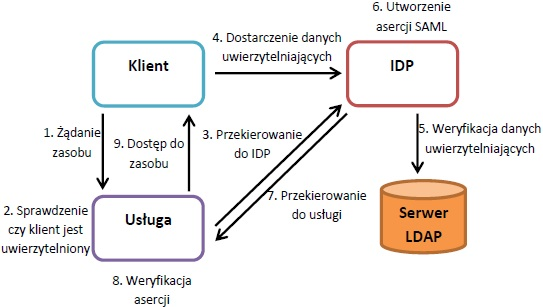
\includegraphics{img/samlWebSSO.jpg}
			\caption{Jednokrotne uwierzytelnianie aplikacji webowych w protokole SAML}
			\label{Jednokrotne uwierzytelnianie aplikacji webowych w protokole SAML}
		\end{figure}

		Podstawowym elementem pozwalającym na realizację procedury jednokrotnego uwierzytelniania dla aplikacji webowych jest usługa "Identity Provider". Usługa odpowiada za uwierzytelnianie klientów oraz dostarcza tożsamości użytkowników do zaufanych aplikacji. IDP wykorzystuje usługę katalogową LDAP jako bazę tożsamości. Dostawcy usług polegają na informacjach na temat użytkowników dostarczanych przez moduł IdP. 

		Kiedy użytkownik chce uzyskać dostęp do zasobów, usługa sprawdza czy klient jest uwierzytelniony. Jeśli nie jest uwierzytelniony następuje przekierowanie do usługi "Identity Provider". Klient podaje swoje dane uwierzytelniające a IDP weryfikuje ich poprawność. Gdy dane są prawidłowe generowana jest asercja SAML i następuje przekierowanie do usługi. Usługa weryfikuje otrzymaną asercję i przydziela lub odmawia prawa dostępu do zasobu. Gdy klient chce uzyskać dostęp do zasobów innej aplikacji nie musi ponownie podawać swoich danych uwierzytelniających, usługa IDP nie dokonuje ponownie procesu uwierzytelniania w usłudze katalogowej LDAP.

%---------------------------------------------------------------------------

\section{Środowisko wdrożenia}
\label{sec:srodowiskoWdrozenia}

Środowisko wdrożenia

%---------------------------------------------------------------------------

\section{Zastosowane mechanizmy integracji}
\label{sec:integracja}

Zastosowane mechanizmy integracji

%---------------------------------------------------------------------------
